\let\negmedspace\undefined
\let\negthickspace\undefined
\documentclass[journal]{IEEEtran}
\usepackage[a5paper, margin=10mm, onecolumn]{geometry}
%\usepackage{lmodern} % Ensure lmodern is loaded for pdflatex
\usepackage{tfrupee} % Include tfrupee package

\setlength{\headheight}{1cm} % Set the height of the header box
\setlength{\headsep}{0mm}     % Set the distance between the header box and the top of the text

\usepackage{gvv-book}
\usepackage{gvv}
\usepackage{cite}
\usepackage{amsmath,amssymb,amsfonts,amsthm}
\usepackage{algorithmic}
\usepackage{graphicx}
\usepackage{textcomp}
\usepackage{xcolor}
\usepackage{txfonts}
\usepackage{listings}
\usepackage{enumitem}
\usepackage{mathtools}
\usepackage{gensymb}
\usepackage{comment}
\usepackage[breaklinks=true]{hyperref}
\usepackage{tkz-euclide} 
\usepackage{listings}
% \usepackage{gvv}                                        
\def\inputGnumericTable{}                                 
\usepackage[latin1]{inputenc}                                
\usepackage{color}                                            
\usepackage{array}                                            
\usepackage{longtable}                                       
\usepackage{calc}                                             
\usepackage{multirow}                                         
\usepackage{hhline}                                           
\usepackage{ifthen}                                           
\usepackage{lscape}
\begin{document}

\bibliographystyle{IEEEtran}
\vspace{3cm}

\title{3-3.3-5}
\author{AI24BTECH11003 - Vijaya Sreyas
}
% \maketitle
% \newpage
% \bigskip
{\let\newpage\relax\maketitle}

\renewcommand{\thefigure}{\theenumi}
\renewcommand{\thetable}{\theenumi}
\setlength{\intextsep}{10pt} % Space between text and floats


\numberwithin{equation}{enumi}
\numberwithin{figure}{enumi}
\renewcommand{\thetable}{\theenumi}


\textbf{Question}:\\
Construct a $\triangle ABC$ in which $CA = 6cm$, $AB = 5cm$ and $BAC = 45\degree$.

\textbf{Solution: }

\begin{table}[h!]    
  \centering
  \begin{tabular}[12pt]{|c|c|l|}
    \hline
	\textbf{Point} & \textbf{Position} & \textbf{Description}\\ 
    \hline
	\textbf{A} & $\myvec{x \\ y}$ & Unknown end of a diameter \\
    \hline 
	\textbf{B} & $\myvec{1 \\ 4}$ & Known end of diameter \\
    \hline
	\textbf{O} & $\myvec{2 \\ -3}$ & Center of the circle \\
    \hline   
    \end{tabular}

  \caption{Given Information}
  \label{3-3.3-5-tab-0}
\end{table}

Using cosine formula in $\triangle ABC$, 
\begin{align}
	a^2 &= b^2 + c^2 - 2bc\cos A \\
	\implies a^2 &= 61 - 30\sqrt{2} \\
\end{align}
The value of a is slightly difficult to work with. To overcome this complication, we can express the coordinates of $\triangle ABC$ as
\begin{align}
        \vec{A} = \vec{O}, \vec{B} = c\myvec{\cos A \\ \sin A}, \vec{C} = \myvec{b \\ 0} \\
        \implies \vec{A} = \vec{O}, \vec{B} = \frac{5}{\sqrt{2}}\myvec{1 \\ 1}, \vec{C} = \myvec{6 \\ 0}
\end{align}
Using these values, we can now plot an example triangle with these sides on a graph.\\

Codes for plotting the triangle:
\begin{lstlisting}
	codes/triangle.c
	codes/plot_triangle.py
\end{lstlisting}

\begin{figure}[H]
    \centering
    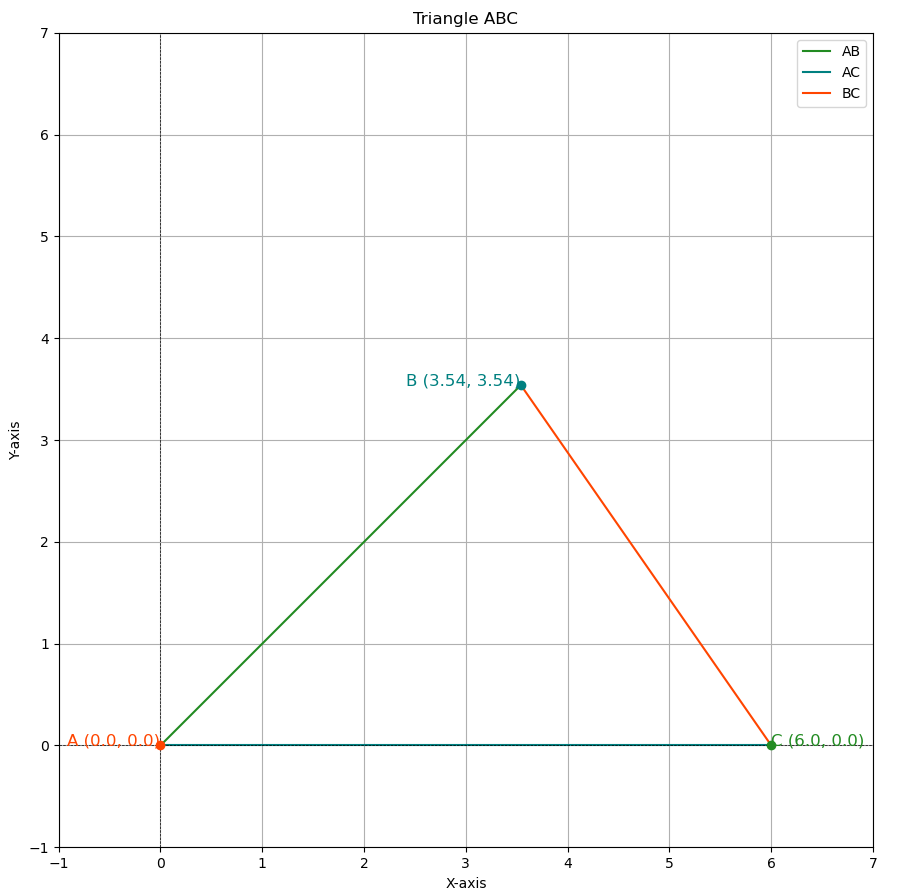
\includegraphics[width=0.7\columnwidth]{figs/Figure_1.png}
    \caption{Plot of the triangle}
    \label{3-3.3-5-fig-0}
\end{figure}

\end{document}


